% P5 paper (M21). Every number comes from numbers.tex (python -m analysis.paper_numbers) or a
% generated table; do not type numbers here (checked by python -m analysis.check_paper).
% Build: tectonic -X compile paper/main.tex
\documentclass[conference]{IEEEtran}
\usepackage[T1]{fontenc}
\usepackage{amsmath,amssymb}
\usepackage{graphicx}
\usepackage{booktabs}
\usepackage{url}
\usepackage[hidelinks]{hyperref}
% generated by `python -m analysis.paper_numbers` from the committed results; do not edit
% \N{key} prints a value; an unknown key is a build error.
\makeatletter
\DeclareRobustCommand{\N}[1]{\@ifundefined{pn@#1}{\errmessage{paper number '#1' undefined}}{\@nameuse{pn@#1}}}
\@namedef{pn@snapshot}{2026-09-21}
\@namedef{pn@rows.compute}{96}
\@namedef{pn@rows.egress}{576}
\@namedef{pn@rows.internet}{24}
\@namedef{pn@rows.storage}{24}
\@namedef{pn@vcpu.aws}{0.0480}
\@namedef{pn@vcpu.azure}{0.0480}
\@namedef{pn@hours}{730}
\@namedef{pn@L.core}{12}
\@namedef{pn@L.ext}{24}
\@namedef{pn@t1.n}{4}
\@namedef{pn@t1.edges}{6}
\@namedef{pn@t1.edgegb}{1,265.50}
\@namedef{pn@t1.netgb}{649.94}
\@namedef{pn@t2.n}{7}
\@namedef{pn@t2.edges}{8}
\@namedef{pn@t2.edgegb}{3,621.00}
\@namedef{pn@t2.netgb}{10.00}
\@namedef{pn@t3.n}{11}
\@namedef{pn@t3.edges}{30}
\@namedef{pn@t3.edgegb}{2,768.94}
\@namedef{pn@t3.netgb}{10,907.14}
\@namedef{pn@tb.runs}{3}
\@namedef{pn@tb.edges}{8}
\@namedef{pn@tb.maxcv}{0.87}
\@namedef{pn@tb.minutes}{10}
\@namedef{pn@tb.users}{20}
\@namedef{pn@tb.rps}{50}
\@namedef{pn@t1.vars}{480}
\@namedef{pn@t1.cons}{76}
\@namedef{pn@t1.ilpsec}{0.0627}
\@namedef{pn@t2.vars}{1,092}
\@namedef{pn@t2.cons}{175}
\@namedef{pn@t2.ilpsec}{0.0768}
\@namedef{pn@t3.vars}{2,292}
\@namedef{pn@t3.cons}{371}
\@namedef{pn@t3.ilpsec}{0.121}
\@namedef{pn@t1.greedy.gap}{0.50}
\@namedef{pn@t1.greedy.sec}{1.12e-04}
\@namedef{pn@t1.onep.gap}{0.50}
\@namedef{pn@t1.onep.sec}{1.48e-04}
\@namedef{pn@t1.sa.gap}{0.00}
\@namedef{pn@t1.sa.sec}{0.278}
\@namedef{pn@t2.greedy.gap}{0.00}
\@namedef{pn@t2.greedy.sec}{1.36e-04}
\@namedef{pn@t2.onep.gap}{0.00}
\@namedef{pn@t2.onep.sec}{2.16e-04}
\@namedef{pn@t2.sa.gap}{0.00}
\@namedef{pn@t2.sa.sec}{0.623}
\@namedef{pn@t3.greedy.gap}{1.83}
\@namedef{pn@t3.greedy.sec}{2.36e-04}
\@namedef{pn@t3.onep.gap}{1.83}
\@namedef{pn@t3.onep.sec}{9.39e-04}
\@namedef{pn@t3.sa.gap}{0.00}
\@namedef{pn@t3.sa.sec}{1.53}
\@namedef{pn@R}{30}
\@namedef{pn@h1.thr}{20}
\@namedef{pn@h1.t1.red}{3.29}
\@namedef{pn@h1.t1.sd}{0.71}
\@namedef{pn@h1.t1.lo}{3.04}
\@namedef{pn@h1.t1.hi}{3.54}
\@namedef{pn@h1.t1.p}{1.000}
\@namedef{pn@h1.t1.b1}{498.00}
\@namedef{pn@h1.t1.ilp}{481.50}
\@namedef{pn@h1.t1.alt}{0.00}
\@namedef{pn@h1.t1.verdict}{REFUTED}
\@namedef{pn@h1.t2.red}{22.55}
\@namedef{pn@h1.t2.sd}{5.81}
\@namedef{pn@h1.t2.lo}{20.52}
\@namedef{pn@h1.t2.hi}{24.59}
\@namedef{pn@h1.t2.p}{0.015}
\@namedef{pn@h1.t2.b1}{1,335.81}
\@namedef{pn@h1.t2.ilp}{1,028.88}
\@namedef{pn@h1.t2.alt}{0.00}
\@namedef{pn@h1.t2.verdict}{SUPPORTED}
\@namedef{pn@h1.t3.red}{1.76}
\@namedef{pn@h1.t3.sd}{0.31}
\@namedef{pn@h1.t3.lo}{1.65}
\@namedef{pn@h1.t3.hi}{1.87}
\@namedef{pn@h1.t3.p}{1.000}
\@namedef{pn@h1.t3.b1}{1,858.56}
\@namedef{pn@h1.t3.ilp}{1,824.64}
\@namedef{pn@h1.t3.alt}{0.00}
\@namedef{pn@h1.t3.verdict}{REFUTED}
\@namedef{pn@h1.verdict}{REFUTED}
\@namedef{pn@h2.maxgap}{5}
\@namedef{pn@h2.minsp}{10}
\@namedef{pn@h2.minn}{15}
\@namedef{pn@h2.minl}{20}
\@namedef{pn@h2.gap}{0.10}
\@namedef{pn@h2.gap.lo}{0.07}
\@namedef{pn@h2.gap.hi}{0.13}
\@namedef{pn@h2.gap.n}{25}
\@namedef{pn@h2.gap.worst}{0.24}
\@namedef{pn@h2.sp}{0.63}
\@namedef{pn@h2.sp.lo}{0.21}
\@namedef{pn@h2.sp.hi}{1.04}
\@namedef{pn@h2.sp.n}{6}
\@namedef{pn@h2.sp.best}{1.04}
\@namedef{pn@h2.verdict}{REFUTED}
\@namedef{pn@h3.points}{9}
\@namedef{pn@h3.smin}{0.01}
\@namedef{pn@h3.smax}{100}
\@namedef{pn@h3.cross}{0}
\@namedef{pn@h3.draws}{30}
\@namedef{pn@h3.rate}{0.00}
\@namedef{pn@h3.rate.hi}{11.35}
\@namedef{pn@h3.allzero}{yes}
\@namedef{pn@h3.verdict}{REFUTED}
\@namedef{pn@sw.t1.ilp}{481.18}
\@namedef{pn@sw.t1.b1}{1,927.49}
\@namedef{pn@sw.t1.pen}{301}
\@namedef{pn@sw.t1.prov}{1}
\@namedef{pn@sw.t2.ilp}{1,028.79}
\@namedef{pn@sw.t2.b1}{28,511.82}
\@namedef{pn@sw.t2.pen}{2,671}
\@namedef{pn@sw.t2.prov}{1}
\@namedef{pn@sw.t3.ilp}{1,789.88}
\@namedef{pn@sw.t3.b1}{1,822.60}
\@namedef{pn@sw.t3.pen}{2}
\@namedef{pn@sw.t3.prov}{1}
\@namedef{pn@sc.nmin}{4}
\@namedef{pn@sc.nmax}{40}
\@namedef{pn@sc.percell}{5}
\@namedef{pn@sc.seeds}{10}
\@namedef{pn@sc.maxsec.core}{10}
\@namedef{pn@sc.maxsec.ext}{46.3}
\@namedef{pn@sc.limit}{600}
\@namedef{pn@tm.repeats}{3}
\@namedef{pn@ab.t1.sa}{0.00}
\@namedef{pn@ab.t1.sa.lo}{0.00}
\@namedef{pn@ab.t1.sa.hi}{0.00}
\@namedef{pn@ab.t1.sb}{-96.44}
\@namedef{pn@ab.t1.sb.lo}{-105.28}
\@namedef{pn@ab.t1.sb.hi}{-88.07}
\@namedef{pn@ab.t1.sc}{112.94}
\@namedef{pn@ab.t1.sc.lo}{103.12}
\@namedef{pn@ab.t1.sc.hi}{123.29}
\@namedef{pn@ab.t2.sa}{0.00}
\@namedef{pn@ab.t2.sa.lo}{0.00}
\@namedef{pn@ab.t2.sa.hi}{0.00}
\@namedef{pn@ab.t2.sb}{107.58}
\@namedef{pn@ab.t2.sb.lo}{91.70}
\@namedef{pn@ab.t2.sb.hi}{124.37}
\@namedef{pn@ab.t2.sc}{199.35}
\@namedef{pn@ab.t2.sc.lo}{176.28}
\@namedef{pn@ab.t2.sc.hi}{223.89}
\@namedef{pn@ab.t3.sa}{0.00}
\@namedef{pn@ab.t3.sa.lo}{0.00}
\@namedef{pn@ab.t3.sa.hi}{0.00}
\@namedef{pn@ab.t3.sb}{-91.95}
\@namedef{pn@ab.t3.sb.lo}{-108.61}
\@namedef{pn@ab.t3.sb.hi}{-77.07}
\@namedef{pn@ab.t3.sc}{125.87}
\@namedef{pn@ab.t3.sc.lo}{108.54}
\@namedef{pn@ab.t3.sc.hi}{144.98}
\@namedef{pn@ab.points}{6}
\@namedef{pn@se.t1.half}{1.99}
\@namedef{pn@se.t1.tq}{2.75}
\@namedef{pn@se.t1.one}{3.50}
\@namedef{pn@se.t1.onehalf}{4.96}
\@namedef{pn@se.t2.half}{14.20}
\@namedef{pn@se.t2.tq}{19.83}
\@namedef{pn@se.t2.one}{24.75}
\@namedef{pn@se.t2.onehalf}{32.94}
\@namedef{pn@se.t3.half}{1.78}
\@namedef{pn@se.t3.tq}{1.78}
\@namedef{pn@se.t3.one}{1.78}
\@namedef{pn@se.t3.onehalf}{1.78}
\@namedef{pn@se.mult.half}{0.5}
\@namedef{pn@se.mult.tq}{0.75}
\@namedef{pn@se.mult.one}{1}
\@namedef{pn@se.mult.onehalf}{1.5}
\@namedef{pn@se.n}{10}
\@namedef{pn@se.k}{4}
\@namedef{pn@s1}{1}
\@namedef{pn@ci}{95}
\@namedef{pn@boot.b}{10,000}
\@namedef{pn@boot.seed}{12345}
\@namedef{pn@smalln}{10}
\@namedef{pn@sa.seeds}{10}
\@namedef{pn@sa.alpha}{0.995}
\@namedef{pn@sa.stale}{20}
\@namedef{pn@sa.prelocate}{80}
\@namedef{pn@sa.probe}{200}
\@namedef{pn@sa.accept}{80}
\@namedef{pn@sa.tmin}{$10^{-4}$}
\@namedef{pn@unc.rate}{0.25}
\@namedef{pn@unc.global}{0.3}
\@namedef{pn@unc.edge}{0.3}
\@namedef{pn@unc.seed}{10,000}
\@namedef{pn@gen.density}{0.25}
\@namedef{pn@gen.median}{200}
\@namedef{pn@runs.rep}{8,100}
\@namedef{pn@runs.scale}{1,250}
\@namedef{pn@runs.abl}{4,320}
\@namedef{pn@runs.sens}{1,800}
\makeatother

\graphicspath{{figures/}}
\newcommand{\pct}[1]{\N{#1}\%}
\newcommand{\usdm}[1]{USD~\N{#1}}
\newcommand{\B}[1]{\textsf{#1}}

\begin{document}

\title{Egress-Aware Cost-Optimal Placement of Multi-Component Workloads Across AWS, Azure and Google Cloud}

\author{%
\IEEEauthorblockN{Aditya Raj}
\IEEEauthorblockA{Reg.\ No.\ 23BCE1052\\
School of Computer Science and Engineering\\
\textit{[Institute name, City]}}
\and
\IEEEauthorblockN{Divyansh Patil}
\IEEEauthorblockA{Reg.\ No.\ 23BCE1506\\
School of Computer Science and Engineering\\
\textit{[Institute name, City]}}
\and
\IEEEauthorblockN{Dr.\ Indrapriyadarshini S}
\IEEEauthorblockA{Project Guide\\
School of Computer Science and Engineering\\
\textit{[Institute name, City]}}}

\maketitle

\begin{abstract}
Public clouds bill outbound data transfer per gigabyte, at a rate that depends on the sending
region and on where the receiver sits. When an application is split into communicating
components, that charge is defined over pairs of locations, so placing each component where its
compute is cheapest ignores a term that can outweigh the saving. We build a dated cost model of
AWS, Azure and Google Cloud from their public price lists, formulate placement as a quadratic
semi-assignment problem with an exact linearisation, and compare it with an egress-aware greedy
heuristic, simulated annealing and two baselines on three application topologies, one with traffic
measured on a local Kubernetes testbed. Over \N{R} paired traffic draws the exact optimum is
\pct{h1.t1.red}, \pct{h1.t2.red} and \pct{h1.t3.red} cheaper than an egress-blind
cheapest-per-vCPU baseline; only the data pipeline clears our pre-registered \pct{h1.thr}
threshold. An ablation attributes the gain to the inter-component egress term. Two further
pre-registered hypotheses are refuted: annealing is within \pct{h2.gap} of the optimum but not
faster than the exact solver, and no traffic-scale crossover between single- and multi-provider
optima exists, because one region minimises every component's own cost in this snapshot.
\end{abstract}

\section{Introduction}
Compute is the line item that teams compare when they choose a cloud region, but it is not the
only one that depends on location. Every provider charges for bytes that leave a region, and the
price depends on whether the receiver is in the same region, another region of the same provider,
or another provider altogether. A multi-component application whose components talk to each other
therefore has a monthly bill whose transfer term is a function of \emph{pairs} of placements. Choosing
each component's location on its own, which is how a price-comparison table is normally used,
optimises a different objective from the one that is billed.

This paper asks how much that difference costs on realistic always-on applications, and whether
an optimiser that prices egress is worth its complexity. We make four contributions, each tied to
a pre-registered objective:
(i)~a unified, dated monthly cost model for AWS, Azure and Google Cloud built only from their public
price lists, with \N{rows.compute} compute, \N{rows.egress} inter-location transfer,
\N{rows.internet} internet-egress and \N{rows.storage} storage rows at snapshot \N{snapshot};
(ii)~an exact integer-programming formulation of egress-coupled placement, with a linearisation
that is provably exact and tighter than the textbook McCormick form;
(iii)~an egress-aware greedy heuristic with local search and a simulated-annealing heuristic, with
their optimality gaps measured against proven optima; and
(iv)~an evaluation of the cost penalty of ignoring egress, with traffic uncertainty propagated into
\N{ci}\% confidence intervals and three hypotheses whose thresholds were frozen before any result existed.

The results are mostly negative, and we report them as such. The penalty of ignoring egress is real
but exceeds our \pct{h1.thr} threshold only on the traffic-heavy pipeline; annealing is accurate but
slower than an exact solver that proves optimality in seconds; and the multi-provider placements that
motivated the project never appear, for a structural reason we identify in the price data.

\section{Related Work}
Prior work on inter-cloud cost falls into four groups, each of which leaves part of our question open.
\emph{Transfer optimisation with fixed endpoints} (gap G1) prices egress carefully but treats the
location of compute as an input: Skyplane plans overlay paths for bulk transfers~\cite{jain2023skyplane},
Cloudcast builds cost-aware multicast trees~\cite{wooders2024cloudcast}, MACARON caches data to cut
cross-cloud reads~\cite{park2024reducing}, SkyStore replicates objects across regions and
clouds~\cite{liu2025skystore}, serverless replication moves object data across
vendors~\cite{shu2026serverless}, and Eliav et~al.\ choose between VPN and dedicated interconnects for
one provider pair~\cite{eliav2026understanding}.
\emph{Component placement without a provider-pair egress tariff} (G2) optimises where microservices run,
but models traffic as a co-location constraint, a per-node coefficient or a per-link cost:
the multi-cloud re-orchestration work of Zambianco et~al.~\cite{zambianco2024cost,zambianco2025disruptionaware},
CaMP-INC~\cite{ali2022campinc} and edge-cloud placement by Kontos et~al.~\cite{kontos2023cloudnative}.
SkyPilot is the closest formulation: its broker solves an ILP over a task DAG and does charge inter-task
egress~\cite{yang2023skypilot}, but for batch tasks run once rather than always-on services with a steady
monthly volume per edge, and without measuring heuristic optimality gaps.
\emph{Workflow scheduling across clouds} (G3) prices transfers between tasks but optimises makespan,
reliability or carbon alongside cost~\cite{tekawade2023cost,christofidi2026huntms}; a survey of the area
is given by Versluis et~al.~\cite{versluis2021a}, and data placement for multi-tenant federations is
studied by Liu et~al.~\cite{liu2021data}.
\emph{Heuristic placement without an exact reference} (G4) is closest in method: Sinha applies hill
climbing and simulated annealing to AWS and Azure pricing~\cite{sinha2023optimization}, but with two
providers, no inter-component transfer term and no exact optimum to measure a gap against.

Our work combines the pieces these groups hold separately: a provider-pair egress tariff on every
directed component edge, three providers at a dated snapshot, an exact optimum, and heuristic gaps
measured against it.

\section{System and Cost Model}
\label{sec:model}
\textbf{Prices.} Three scripts pull the AWS Price List bulk API, the Azure Retail Prices API and
Google Cloud's published price pages for Linux, on-demand, shared-tenancy compute; block and object
storage; and outbound transfer. The \emph{core} location set has four regions per provider
(\N{L.core} in all) and the \emph{extended} set has eight (\N{L.ext}), used only for scaling.
Each component has a fixed instance shape, the smallest meeting its vCPU and memory requirement,
so the only decision is its location. A month is \N{hours} hours. Tiered egress prices are
flattened to the first paid tier, free allowances are ignored, and every validation rule of the
cost model (non-negative prices, zero same-region transfer, a complete location-pair matrix)
passes with no fallback rates.

\textbf{Cost of an assignment.} For components $C$, locations $L$ and an assignment $a: C\to L$,
\begin{equation}
\mathcal{C}(a)=\sum_{c\in C} k_{c,a(c)}+\sum_{(u,v)\in E} w_{uv}\,p_{a(u),a(v)}+\sum_{c\in C} q_c\,r_{a(c)},
\label{eq:cost}
\end{equation}
where $k_{c\ell}$ is the monthly compute plus storage cost of $c$ at $\ell$, $w_{uv}$ the monthly
traffic in GB on directed edge $(u,v)$, $p_{\ell m}$ the per-GB price of sending from $\ell$ to
$m$ (paid by the sender, $p_{\ell\ell}=0$), $q_c$ the traffic from $c$ to end users and $r_\ell$
the internet egress price at $\ell$. One function implements~(\ref{eq:cost}), and every method in
this paper, baselines included, is costed by it; a test asserts that the exact solver's objective
equals this function on its own assignment.

\textbf{Two facts in the snapshot.} AWS \texttt{us-east-1} and Azure \texttt{eastus} charge exactly
the same per vCPU-hour (USD~\N{vcpu.aws}) for every shape we use, and Azure \texttt{eastus} alone
minimises the \emph{own} cost $k_{c\ell}+q_c r_\ell$ of every component of all three topologies.
Both facts shape the results in Section~\ref{sec:eval}.

\section{Problem Formulation}
\label{sec:ilp}
The middle term of~(\ref{eq:cost}) couples pairs of placements, making the problem a quadratic
semi-assignment problem. Let $x_{c\ell}\in\{0,1\}$ place $c$ at $\ell\in A_c$, where $A_c=L$ unless
$c$ is pinned. Merge the two directions of each connected pair $\{u,v\}\in P$ into
$W_{uv}(\ell,m)=w_{uv}p_{\ell m}+w_{vu}p_{m\ell}$, and introduce continuous $y_{uv\ell m}\ge 0$
standing for $x_{u\ell}x_{vm}$. The model is
\begin{align}
\min\;& \sum_{c}\sum_{\ell\in A_c}\bigl(k_{c\ell}+q_c r_\ell\bigr)x_{c\ell}
       +\sum_{\{u,v\}\in P}\sum_{\ell\in A_u}\sum_{m\in A_v}W_{uv}(\ell,m)\,y_{uv\ell m}\nonumber\\
\text{s.t.}\;& \textstyle\sum_{\ell\in A_c}x_{c\ell}=1 \quad \forall c\in C,\label{eq:assign}\\
& \textstyle\sum_{m\in A_v}y_{uv\ell m}=x_{u\ell}\quad \forall\{u,v\}\in P,\ \ell\in A_u,\label{eq:row}\\
& \textstyle\sum_{\ell\in A_u}y_{uv\ell m}=x_{vm}\quad \forall\{u,v\}\in P,\ m\in A_v.\label{eq:col}
\end{align}

\textbf{Exactness.} Fix an integer $x$ satisfying~(\ref{eq:assign}) with $a(u)=\ell^*$ and
$a(v)=m^*$, and read $y_{uv}$ as a non-negative $|A_u|\times|A_v|$ matrix. Every row
$\ell\ne\ell^*$ sums to zero by~(\ref{eq:row}), so it vanishes; every column $m\ne m^*$ vanishes
by~(\ref{eq:col}); the single remaining entry $y_{uv\ell^*m^*}$ equals one. Hence
$y_{uv\ell m}=x_{u\ell}x_{vm}$ for every feasible integer $x$, independently of the objective,
and the model's objective is exactly~(\ref{eq:cost}).

\textbf{Tightness.} In the LP relaxation, (\ref{eq:row})--(\ref{eq:col}) imply the McCormick
inequalities $y_{uv\ell m}\ge x_{u\ell}+x_{vm}-1$ and $y\le x$, but not conversely: with every
$x_{c\ell}=1/|L|$ McCormick admits $y\equiv 0$, which erases all transfer cost from the bound.
This is the standard assignment (RLT) linearisation; we keep McCormick only as an ablation. With no
pins the model has $n|L|$ binaries, $|P||L|^2$ continuous variables and $n+2|P||L|$ constraints;
on the core set T1, T2 and T3 have \N{t1.vars}, \N{t2.vars} and \N{t3.vars} variables and
\N{t1.cons}, \N{t2.cons} and \N{t3.cons} constraints. We solve with CBC through PuLP, single-threaded,
with a \N{sc.limit}\,s limit, and read optimality from CBC's own log because PuLP labels a run
stopped on the time limit as optimal.

\section{Heuristics and Baselines}
\label{sec:heur}
\textbf{Greedy and 1-opt.} The greedy heuristic places components in decreasing order of total
incident traffic, each at the location minimising its own cost plus the transfer cost to and from
the components already placed. The 1-opt local search then relocates single components while any
move lowers~(\ref{eq:cost}).

\textbf{Simulated annealing (SA).} The state is a full assignment, initialised from greedy. A move
relocates one component (probability \pct{sa.prelocate}) or swaps two; its cost change is computed
incrementally from incident edges. The initial temperature is calibrated so that about
\pct{sa.accept} of uphill moves in a \N{sa.probe}-move probe are accepted; cooling is geometric
with $\alpha=\N{sa.alpha}$ every $n|L|$ moves, and a run stops when the temperature falls below
\N{sa.tmin} of its initial value or after \N{sa.stale} consecutive temperature steps without
improvement. SA returns the best assignment it visited.

\textbf{Baselines.} \B{B1} (cheapest-per-vCPU, independent) places each component, on its own, at
the location minimising hourly price per vCPU for its shape; egress is ignored when choosing but
charged when evaluating. Because AWS \texttt{us-east-1} and Azure \texttt{eastus} tie on that
price, B1 needs a tie-break: we report B1 with the component's storage bill as tie-break and
\B{B1-alt} with the opposite choice as a robustness check. \B{B2} (single provider) puts every
component in one provider's cheapest region for the application's compute and storage bill;
\B{B2-best} is the cheapest of the three.

\section{Experimental Setup}
\label{sec:setup}
\textbf{Workloads.} T1 is a three-tier web application (\N{t1.n} components, \N{t1.edges} directed
edges). Its traffic was measured on a single-node \texttt{kind} Kubernetes cluster on a laptop:
\N{tb.runs} locust runs of \N{tb.minutes} minutes each with \N{tb.users} users, with every edge's
TCP payload counted at the socket, scaled to \N{tb.rps} requests/s; the largest coefficient of
variation of bytes per request across runs is \pct{tb.maxcv}. This gives \N{t1.edgegb}~GB/month
between components and \N{t1.netgb}~GB/month to users. T2 is a data pipeline (\N{t2.n} components,
\N{t2.edgegb}~GB/month between components) and T3 an Online-Boutique-shaped microservice
application (\N{t3.n} components, \N{t3.edges} edges, \N{t3.edgegb}~GB/month), both with stated
volumes. No cloud resource was created at any point.

\textbf{Uncertainty and replication.} Each result is replicated over $R=\N{R}$ traffic draws, and
every method is solved on the same draw, so comparisons are paired. For T1 we resample the measured
per-run bytes per request and apply a shared request-rate factor $e^{Z}$, $Z\sim\mathcal{N}(0,\N{unc.rate}^2)$;
for T2 and T3 every edge is multiplied by a shared load factor and an independent per-edge factor,
both lognormal with $\sigma=\N{unc.global}$. Prices are held fixed at the snapshot. Intervals are
\N{ci}\% percentile bootstrap intervals with $B=\N{boot.b}$ resamples (the wider of bootstrap and $t$
below \N{smalln} values); proportions use Wilson intervals. Altogether the replicated experiments
ran \N{runs.rep} traffic-draw jobs, \N{runs.scale} scaling jobs, \N{runs.abl} ablation jobs and
\N{runs.sens} sensitivity jobs.

\textbf{Traffic sweep.} Every inter-component volume is multiplied by a scale $s$ over
\N{h3.points} log-spaced points from \N{h3.smin} to \N{h3.smax}; $s=\N{s1}$ is the measured or
stated traffic.

\textbf{Scaling.} Synthetic instances with $n=\N{sc.nmin}$ to \N{sc.nmax} components (edge density
\N{gen.density}, lognormal volumes with median \N{gen.median}~GB/month), \N{sc.percell} per cell,
on both location sets; SA uses \N{sc.seeds} seeds per instance and runtimes are means of
\N{tm.repeats} timing repeats on one machine.

\textbf{Hypotheses (frozen).} \emph{H1:} at $s=\N{s1}$ the ILP reduces cost by at least
\pct{h1.thr} relative to B1. \emph{H2:} at $n\ge\N{h2.minn}$ and $|L|\ge\N{h2.minl}$, on instances
CBC solves to proven optimality, SA's median gap is at most \pct{h2.maxgap} \emph{and} it is at least
\N{h2.minsp}$\times$ faster. \emph{H3:} a traffic scale exists above which the optimum uses a single
provider while B1 stays multi-provider, with the ordering inverted below it. A hypothesis is SUPPORTED
only if the whole confidence interval clears its threshold, REFUTED if the whole interval misses it,
and INCONCLUSIVE otherwise.

\section{Evaluation}
\label{sec:eval}

\begin{table}[t]
\centering
\caption{Monthly cost at $s=\N{s1}$ and the H1 reduction $\rho=(C(\mathrm{B1})-C(\mathrm{ILP}))/C(\mathrm{B1})$.
Mean over $R=\N{R}$ paired traffic draws; $\rho$ as mean $\pm$ sd with its \N{ci}\% bootstrap CI;
$p$ is the one-sided Wilcoxon test of $\rho>\pct{h1.thr}$. Snapshot \N{snapshot}, core set.}
\label{tab:h1}
\setlength{\tabcolsep}{3.5pt}
\begin{tabular}{lrrlrl}
\toprule
 & B1 & ILP & $\rho$, \% (\N{ci}\% CI) & $p$ & H1 \\
 & USD/mo & USD/mo & & & \\
\midrule
T1 & \N{h1.t1.b1} & \N{h1.t1.ilp} & \N{h1.t1.red} $\pm$ \N{h1.t1.sd} [\N{h1.t1.lo}, \N{h1.t1.hi}] & \N{h1.t1.p} & \N{h1.t1.verdict} \\
T2 & \N{h1.t2.b1} & \N{h1.t2.ilp} & \N{h1.t2.red} $\pm$ \N{h1.t2.sd} [\N{h1.t2.lo}, \N{h1.t2.hi}] & \N{h1.t2.p} & \N{h1.t2.verdict} \\
T3 & \N{h1.t3.b1} & \N{h1.t3.ilp} & \N{h1.t3.red} $\pm$ \N{h1.t3.sd} [\N{h1.t3.lo}, \N{h1.t3.hi}] & \N{h1.t3.p} & \N{h1.t3.verdict} \\
\bottomrule
\end{tabular}
\end{table}

\begin{figure*}[t]
\centering
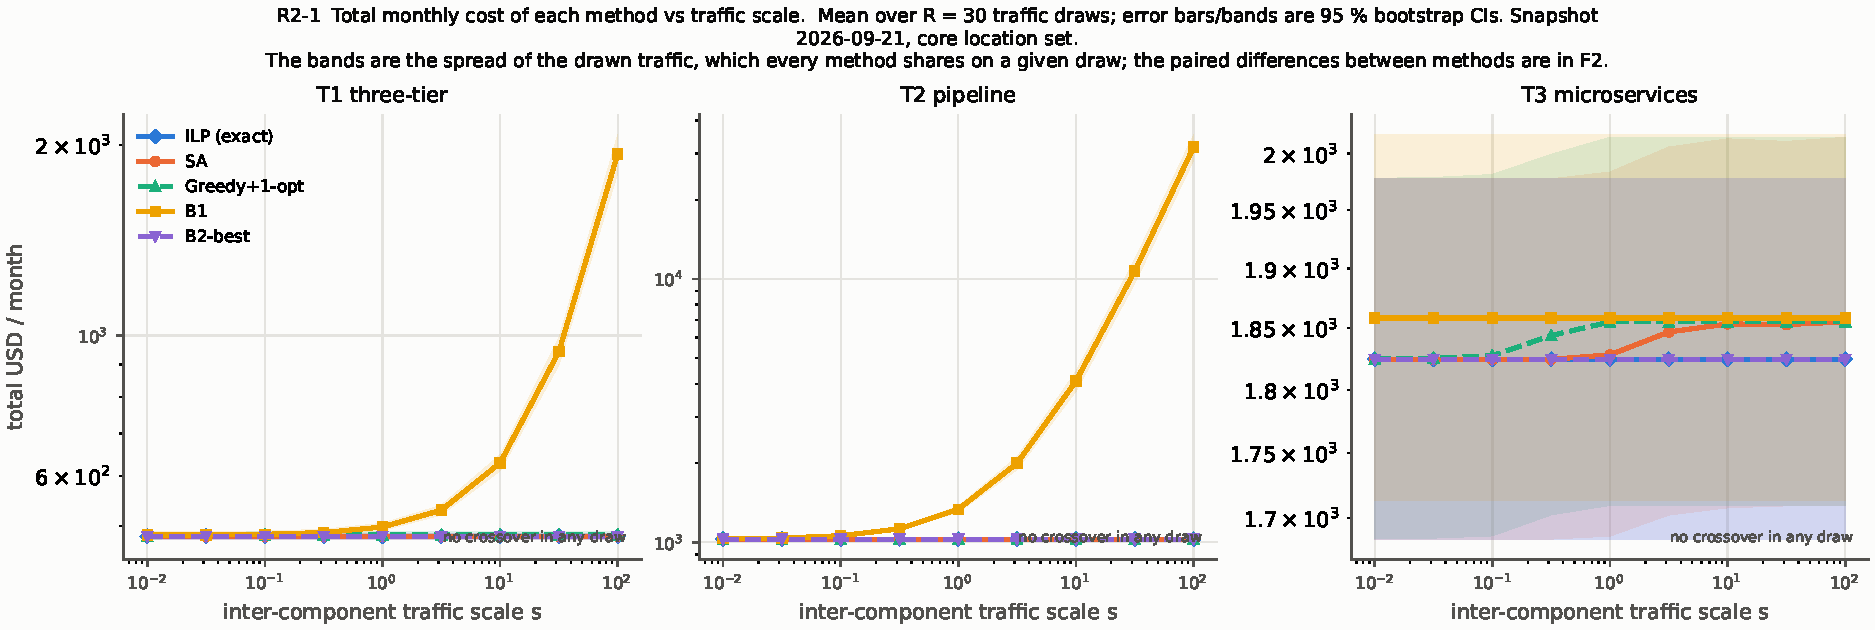
\includegraphics[width=\textwidth]{R2-1_cost_vs_scale.pdf}
\caption{Total monthly cost of each method against the inter-component traffic scale $s$ on T1--T3.
Mean over $R=\N{R}$ traffic draws ($n=\N{R}$ per point); error bands are \N{ci}\% bootstrap CIs.
Snapshot \N{snapshot}, core location set.}
\label{fig:r21}
\end{figure*}

\subsection{Cost of each method and the size of the gain (H1)}
Table~\ref{tab:h1} and Fig.~\ref{fig:r21} give the headline. The exact ILP, proven optimal by CBC on
every solve, costs \usdm{h1.t1.ilp}, \usdm{h1.t2.ilp} and \usdm{h1.t3.ilp} per month on T1, T2 and
T3 and coincides with B2-best: the optimum is single-provider. B1 costs more because its storage
tie-break splits T1 and T2 across two providers, which then pay inter-component egress. The paired
reduction is \pct{h1.t1.red}, \pct{h1.t2.red} and \pct{h1.t3.red}. Only T2's interval
[\pct{h1.t2.lo}, \pct{h1.t2.hi}] lies above the \pct{h1.thr} threshold, and narrowly, so
\textbf{H1 is \N{h1.verdict} overall and SUPPORTED on T2 alone}. Under the opposite tie-break
(B1-alt) B1 already places everything in Azure \texttt{eastus} and the reduction is \pct{h1.t1.alt}
on every topology; the verdict therefore does not rest on a tie-break chosen in the method's favour.
Fig.~\ref{fig:f1} shows where the money goes: compute dominates T1 and T2 and internet egress to
users dominates T3; B1's excess is mostly inter-component egress on T1 and T2, while on T3, which B1
places entirely in AWS, it is the higher internet egress price there.

\begin{figure*}[t]
\centering
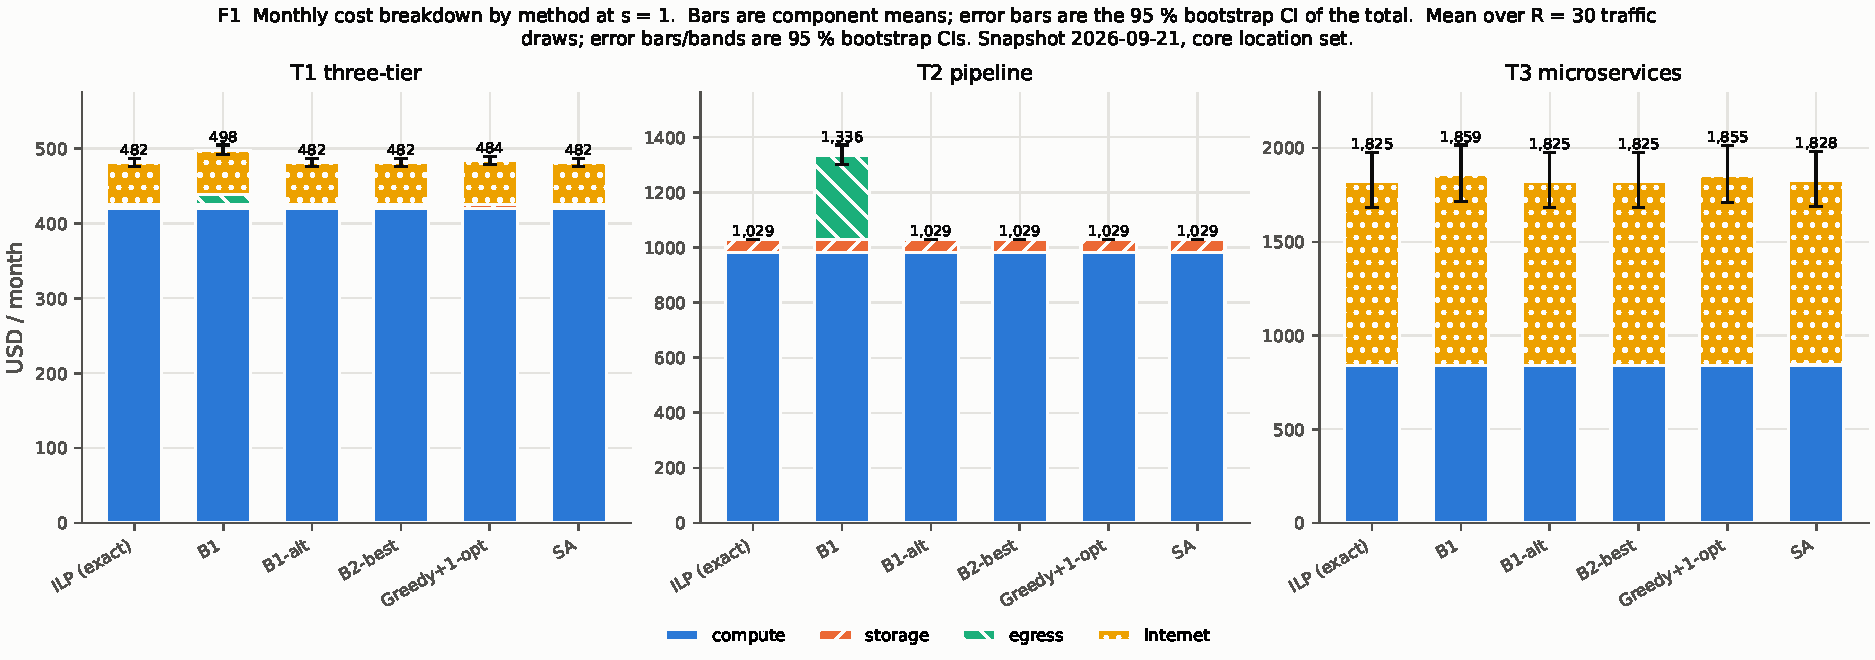
\includegraphics[width=0.92\textwidth]{F1_cost_breakdown.pdf}
\caption{Monthly cost breakdown by method at $s=\N{s1}$ into compute, storage, inter-component egress
and internet egress. Bars are component means over $R=\N{R}$ traffic draws ($n=\N{R}$); error bars are
the \N{ci}\% bootstrap CI of the total. Snapshot \N{snapshot}, core location set.}
\label{fig:f1}
\end{figure*}

\subsection{Where the gain comes from (ablation)}
We decompose $G=C(\mathrm{B1})-C(\mathrm{ILP})$ into three steps that add one cost term at a time to
the objective the optimiser sees (Fig.~\ref{fig:f6}). Pricing storage alongside compute buys
\usdm{ab.t1.sa} on every topology, since B1's tie-break already picks the cheapest storage. Adding
internet egress alone is \emph{negative} on T1 (\usdm{ab.t1.sb}, CI [\N{ab.t1.sb.lo}, \N{ab.t1.sb.hi}])
and T3 (\usdm{ab.t3.sb}): an optimiser that sees user traffic but not inter-component traffic moves
components apart and makes the true bill worse. The third step, pricing inter-component egress,
recovers \usdm{ab.t1.sc} on T1, \usdm{ab.t2.sc} on T2 and \usdm{ab.t3.sc} on T3 and is the largest
step at all \N{ab.points} (topology, scale) points. The optimiser's value is specifically the egress
coupling, not better unit-price shopping.

\begin{figure*}[t]
\centering
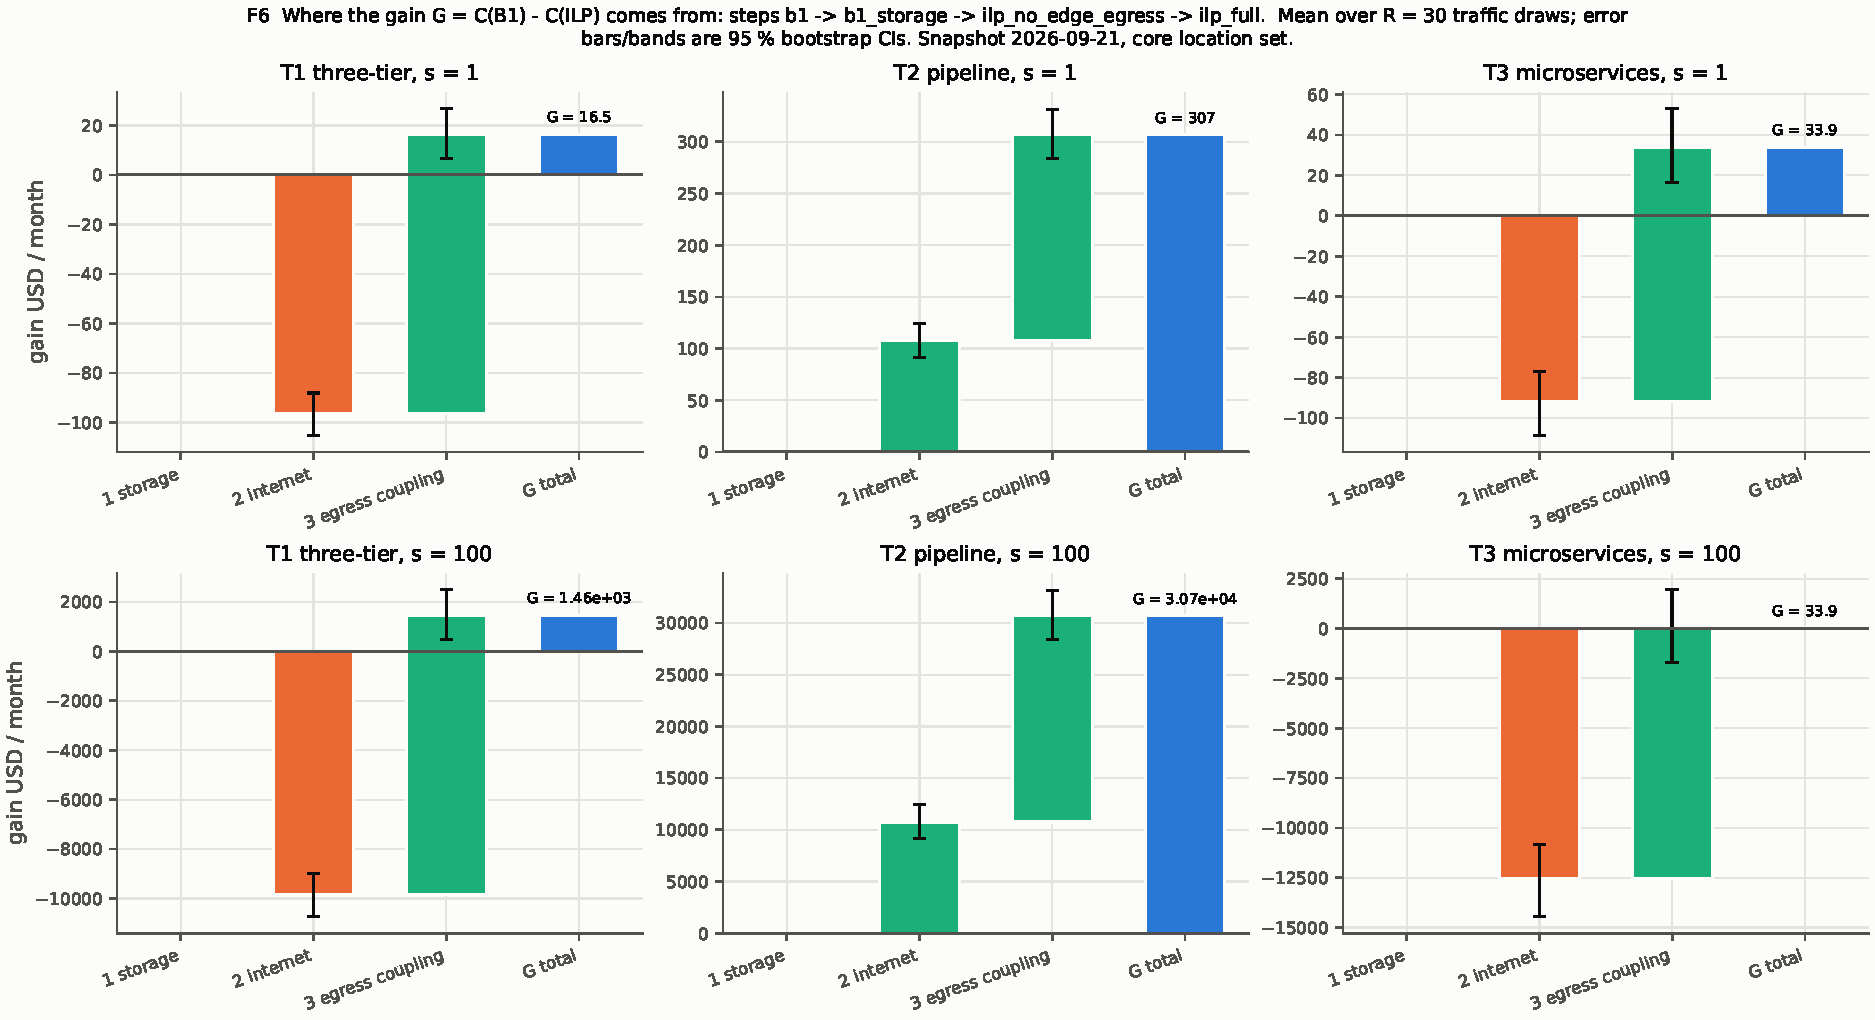
\includegraphics[width=0.92\textwidth]{F6_gain_decomposition.pdf}
\caption{Decomposition of the gain $G=C(\mathrm{B1})-C(\mathrm{ILP})$ into the steps b1 $\to$ b1\_storage
$\to$ ilp\_no\_edge\_egress $\to$ ilp\_full, per topology and traffic scale. Mean over $R=\N{R}$ traffic
draws ($n=\N{R}$ per bar); error bars are \N{ci}\% bootstrap CIs of each step. Snapshot \N{snapshot},
core location set.}
\label{fig:f6}
\end{figure*}

\subsection{Traffic sweep and the crossover (H3)}
As $s$ grows, B1's penalty grows steeply on T1 and T2 (Fig.~\ref{fig:r21}): at $s=\N{h3.smax}$ on
T2 B1 costs \usdm{sw.t2.b1} per month against an unchanged optimum of \usdm{sw.t2.ilp}, a penalty of
\N{sw.t2.pen}\%. But the optimum never uses more than one provider. In \N{h3.cross} of \N{h3.draws}
draws on each topology does a crossover appear (rate \pct{h3.rate}, Wilson \N{ci}\% CI
[\pct{h3.rate}, \pct{h3.rate.hi}]), and \textbf{H3 is \N{h3.verdict} on all three topologies}.
This is structural, not a matter of grid resolution. Because Azure \texttt{eastus} minimises every
component's own cost, and inter-component egress is non-negative and zero when components share a
location, placing everything there is optimal at \emph{every} $s\ge 0$ in this snapshot. A crossover
requires components whose own-cost minimisers differ, for example one pinned to another provider by a
data-residency rule.

\subsection{Exact frontier and heuristic quality (H2)}
On T1--T3 at $s=\N{s1}$ CBC proves optimality in \N{t1.ilpsec}, \N{t2.ilpsec} and \N{t3.ilpsec}\,s.
Greedy's gap is \pct{t1.greedy.gap}, \pct{t2.greedy.gap} and \pct{t3.greedy.gap}; 1-opt does not
improve it, and SA reaches the optimum (median over \N{sa.seeds} seeds) on all three, with a median runtime of
\N{t3.sa.sec}\,s on T3.

On the synthetic instances CBC proved optimality everywhere up to $n=\N{sc.nmax}$ on both location
sets, so the exact frontier was \emph{not} reached; the slowest solve took \N{sc.maxsec.ext}\,s
against a \N{sc.limit}\,s limit (Fig.~\ref{fig:f4}). In the qualifying cells SA's median gap is
\pct{h2.gap} over \N{h2.gap.n} instances (CI [\pct{h2.gap.lo}, \pct{h2.gap.hi}], worst instance
\pct{h2.gap.worst}), well inside the \pct{h2.maxgap} accuracy clause (Fig.~\ref{fig:f5}). The speed-up
clause fails: over \N{h2.sp.n} timed instances SA's median speed-up over CBC is \N{h2.sp}$\times$
(CI [\N{h2.sp.lo}, \N{h2.sp.hi}]$\times$, best \N{h2.sp.best}$\times$) against the required
\N{h2.minsp}$\times$. \textbf{H2 is \N{h2.verdict}}: the tight formulation makes the exact solver fast
enough that annealing has nothing to save at these sizes. Greedy runs in milliseconds but its gap is
far less predictable.

\begin{figure}[t]
\centering
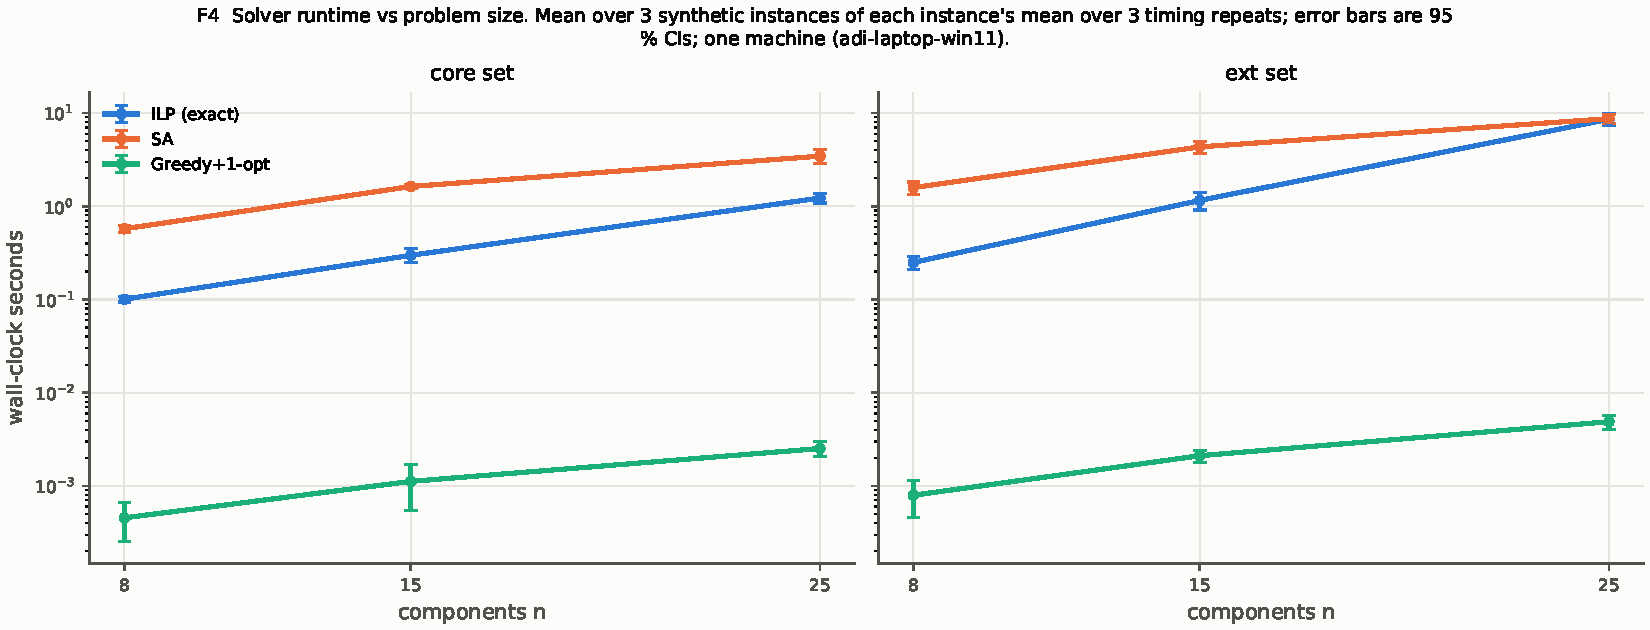
\includegraphics[width=\columnwidth]{F4_runtime_vs_n.pdf}
\caption{Solver runtime against problem size $n$ on the core and extended sets, log scale. Mean over
\N{sc.percell} synthetic instances per point ($n=\N{sc.percell}$), each the mean of \N{tm.repeats}
timing repeats; error bars are \N{ci}\% CIs. One machine; snapshot \N{snapshot}.}
\label{fig:f4}
\end{figure}

\begin{figure}[t]
\centering
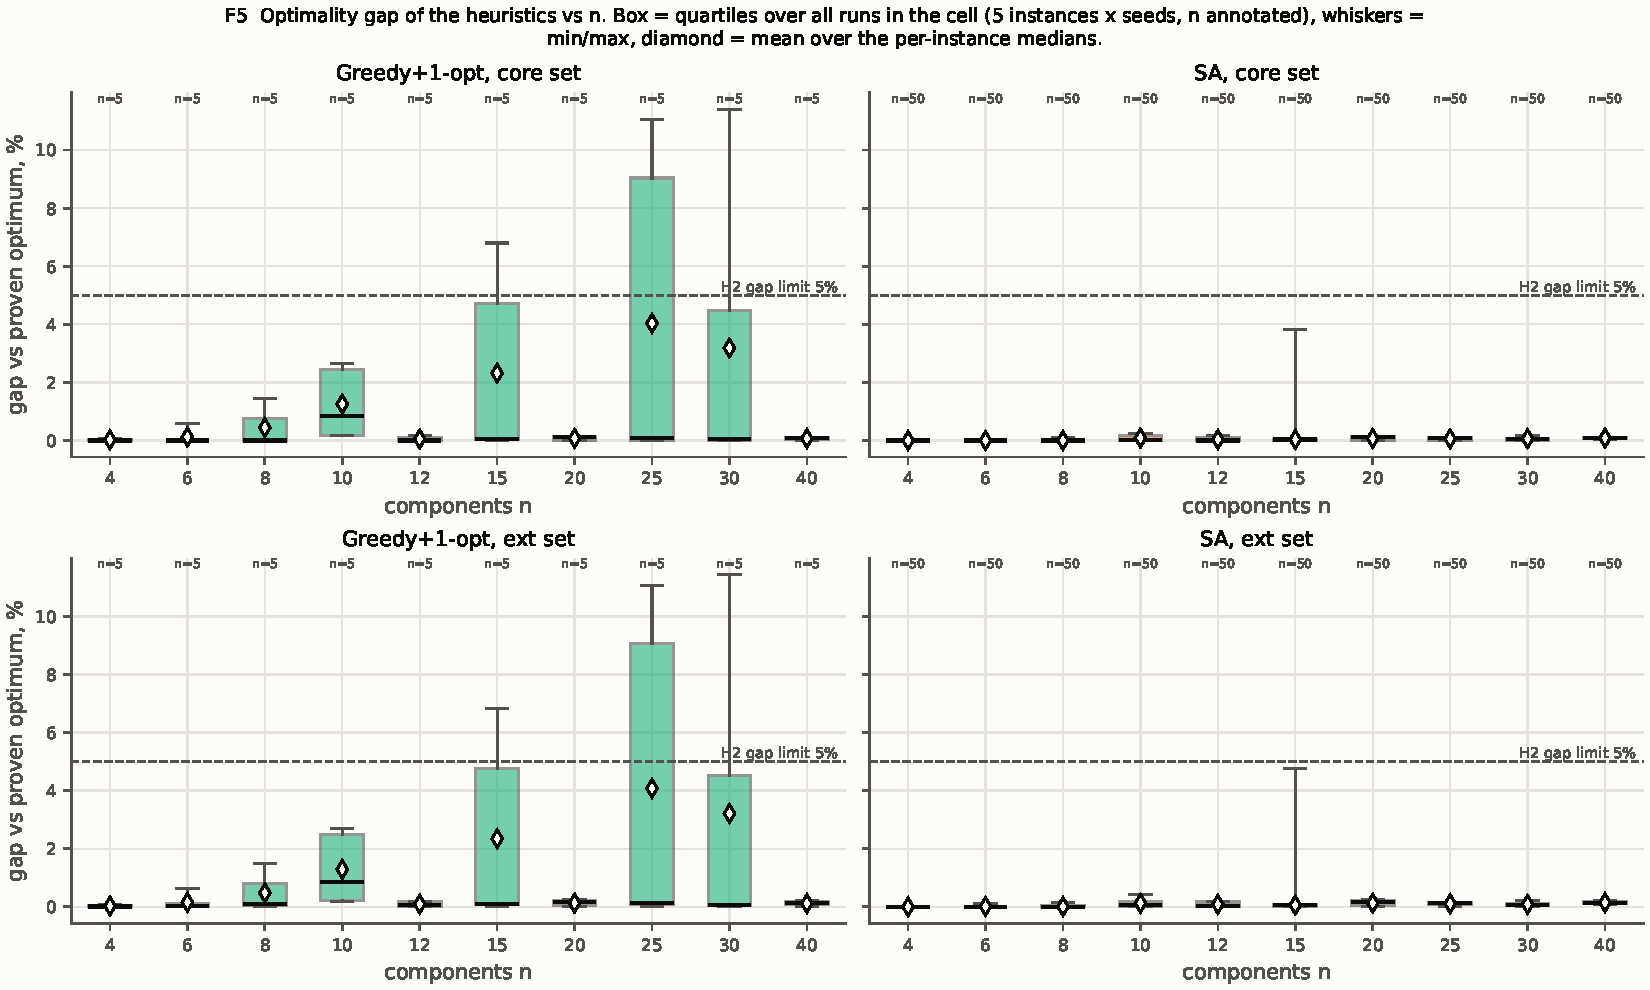
\includegraphics[width=\columnwidth]{F5_gap_boxplots.pdf}
\caption{Optimality gap of SA and greedy with 1-opt against the proven optimum, by $n$ and location set.
Boxes are quartiles over all runs in a cell ($n=\N{sc.percell}$ instances $\times$ \N{sc.seeds} SA
seeds; run counts annotated in the panel), whiskers min/max, diamond the mean of per-instance medians; the H2 gap is reported with its
\N{ci}\% bootstrap CI in the text. Snapshot \N{snapshot}.}
\label{fig:f5}
\end{figure}

\subsection{Sensitivity to prices}
A separate grid of \N{se.n} draws per point (so its values differ slightly from Table~\ref{tab:h1})
varies two features of the price world. Scaling every cross-provider egress price by
$\times\N{se.mult.half}$ to $\times\N{se.mult.onehalf}$ moves T2's saving from \pct{se.t2.half} to \pct{se.t2.onehalf}, crossing the \pct{h1.thr} threshold
between $\times\N{se.mult.tq}$ (\pct{se.t2.tq}) and $\times\N{se.mult.one}$ (\pct{se.t2.one})
(Fig.~\ref{fig:f7}): T2's SUPPORTED verdict would not survive a quarter cut in egress prices.
T1 and T3 stay far below the threshold across the range (\pct{se.t1.onehalf} and \pct{se.t3.onehalf}
at $\times\N{se.mult.onehalf}$). Offering each provider more regions changes almost nothing, because
the winning region is already in the smallest set.

\begin{figure}[t]
\centering
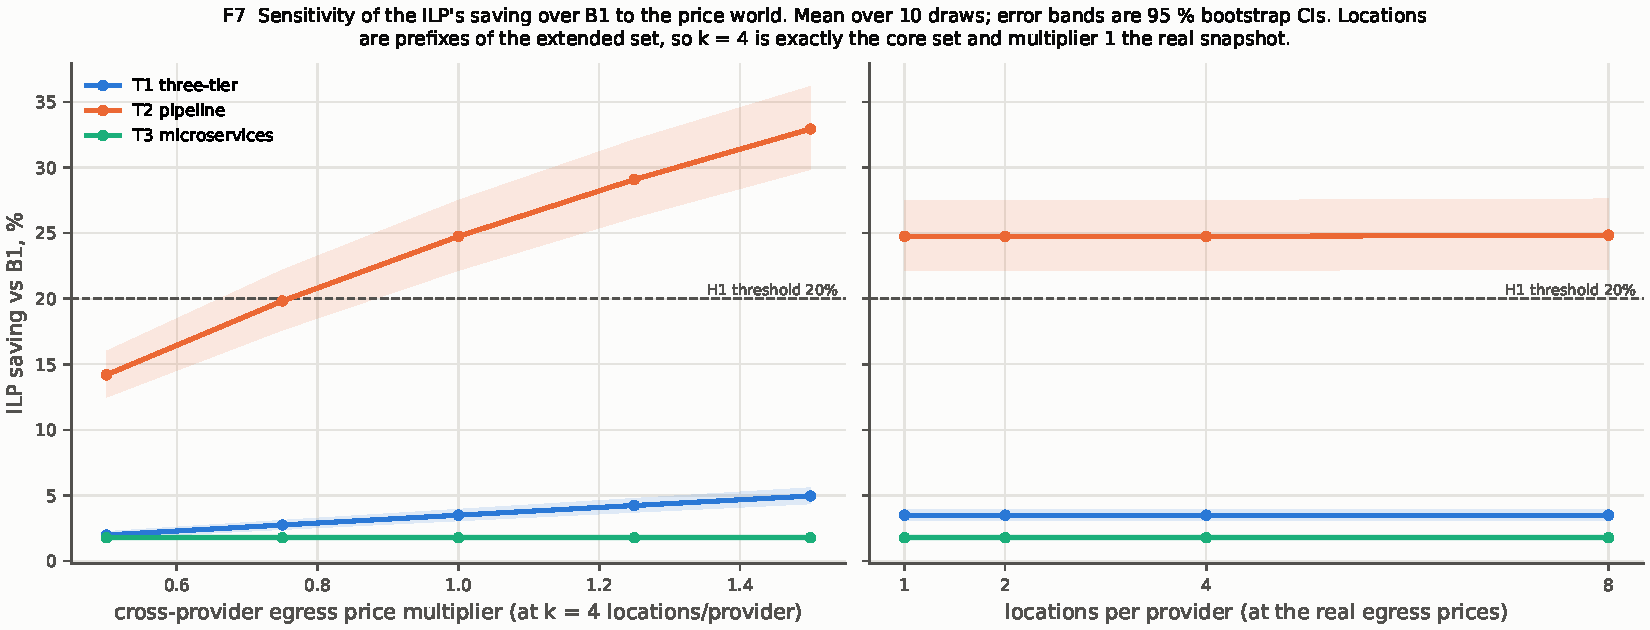
\includegraphics[width=\columnwidth]{F7_sensitivity.pdf}
\caption{Saving of the ILP over B1 against a cross-provider egress-price multiplier (at \N{se.k}
locations per provider) and against the number of locations per provider (at real prices). Mean over
\N{se.n} traffic draws ($n=\N{se.n}$ per point); error bars are \N{ci}\% bootstrap CIs; dashed line at
the \pct{h1.thr} H1 threshold. Snapshot \N{snapshot}.}
\label{fig:f7}
\end{figure}

\section{Threats to Validity}
\label{sec:threats}
Table~\ref{tab:threats} summarises the main threats in the four standard categories, with the
direction in which each biases the reported gain; the full register, with mitigations and residual
risk, is in the repository.

\begin{table}[t]
\centering
\caption{Main threats to validity and the direction of their bias on the reported gain.}
\label{tab:threats}
\footnotesize
\begin{tabular}{p{0.17\columnwidth}p{0.55\columnwidth}p{0.17\columnwidth}}
\toprule
Category & Threat & Bias \\
\midrule
Construct & List price is not the bill: sustained-use discounts, savings plans and free egress allowances are ignored; payload bytes, not wire bytes. & either way \\
Internal & Tiered egress flattened to the first paid tier; cross-zone transfer ignored; shapes fixed per component; SA tuned on a subset. & overstates \\
External & Three topologies and synthetic graphs; one price snapshot; no private interconnects or CDN; no latency, SLO or residency constraints. & overstates \\
Conclusion & Uncertainty models for stated volumes are assumptions; bootstrap over \N{R} draws; runtimes on one laptop; three topologies tested separately. & either way \\
\bottomrule
\end{tabular}
\end{table}

The most consequential threat is the absence of latency, SLO and data-residency constraints.
Such constraints would forbid the colocation that makes the single-region optimum possible, and
they are the setting in which multi-provider placements and a crossover could appear. The second is
the single snapshot: the T2 result is fragile to a modest change in egress prices (Fig.~\ref{fig:f7}),
so a later snapshot could move it either way.

\section{Conclusion}
For three always-on applications priced at one dated snapshot of AWS, Azure and Google Cloud, an exact
egress-aware placement is never worse than the baselines and saves
\pct{h1.t3.red}--\pct{h1.t2.red} over egress-blind cheapest-per-vCPU placement. The saving clears a
pre-registered \pct{h1.thr} bar only for the traffic-heavy pipeline, and all of it comes from pricing
inter-component egress. The optimiser is worth having as protection against egress-blind choices, not
as a way to find multi-cloud splits: in this snapshot one region is cheapest for every component, so
the optimum is always single-provider and no crossover exists. The tight linearisation keeps the exact
problem easy up to $n=\N{sc.nmax}$, which removes the case for annealing at these sizes. The natural
next step is a constrained study, with latency or residency rules that forbid colocation, where the
coupling term would have to be traded against them.

\bibliographystyle{IEEEtran}
\bibliography{refs}

\end{document}
